\RequirePackage{mmap}
\documentclass[12pt]{article}
\usepackage[utf8]{inputenc}
\usepackage{geometry}
\geometry{
  margin=1in,
}
\usepackage{amsmath,amsthm,amssymb, listings, color, bm}
\usepackage{mathtools}
\usepackage{changepage}% http://ctan.org/pkg/changepage
\usepackage{enumitem}
\usepackage{csquotes}
\usepackage{fancyhdr}
\usepackage[T1]{fontenc}
\usepackage{titlesec}
\usepackage[absolute]{textpos}
\usepackage[hidelinks]{hyperref}
\usepackage{fontspec}
\usepackage[linesnumbered,ruled]{algorithm2e}
\setmainfont{Latin Modern Roman}
%% \usepackage{setspace}
%% \doublespacing

\setlength{\parindent}{0.25in}
\setlength{\parskip}{0.5em}

\newif\ifextra
\extrafalse

\title{}

\pagenumbering{arabic}

\begin{document}
\pagestyle{fancy}
\fancyhf{} % sets both header and footer to nothin
\cfoot{\thepage}
\renewcommand{\headrulewidth}{1pt}
\lhead{\fontsize{10}{12} \selectfont CSE 446: Machine Learning (Prof. Sham Kakade)\\\textbf{\emph{Section 3: Perceptron, Bayesian Optimal Classifier, Basics}} }
\rhead{\fontsize{10}{12} \selectfont Kaiyu Zheng (TA)\\ \today}

This is my preperation notes for teaching in sections during the winter 2018 quarter for course CSE 446. Useful for myself to review the concepts as well.

\section{Perceptron}

Perceptron is one of the simplest (linear) binary classifiers. Suppose we observe data points $(x_i, y_i)$ for $i=1,\cdots,N$, where $x_i\in\mathbb{R}^d$ and $y_i\in\{-1,+1\}$. We hope to train the weights $w\in\mathbb{R}^d$ and bias $b$ in the following classification function:
\begin{align}
\hat{y}=f(x)=\text{sign}(w\cdot x+b)
\end{align}
To minimize a loss function $L(w) = \frac{1}{N}\sum_{i=1}^N\ell(y_i, \hat{y})$. The perceptron algorithm is an iterative process, either offline or online. See Algorithm \ref{alg:perceptron-online} and \ref{alg:perceptron-offline}.


\begin{algorithm}[h]
    \caption{Perceptron-Online(T)}
    \label{alg:perceptron-online}
    $w^{(1)}\gets \bm{0}$; $b^{(1)}\gets 0$\;
    \ForEach{$t=1,\cdots,T$}{
      $(x_t, y_t)\gets$ new observation at time $t$\;
      $\hat{y}_t\gets f(w^{(t)}\cdot x_t)$\;
      \If{$\hat{y}_t\neq y_t$}{
        $w^{(t+1)}\gets w^{(t)}+y_tx_t$\;
        $b^{(t+1)}\gets b^{(t)}+y_t$
      }
    }
\end{algorithm}

\begin{algorithm}[h]
    \caption{Perceptron-Offline$(\mathcal{D},T)$}
    \label{alg:perceptron-offline}
    $w^{(1)}\gets \bm{0}$; $b^{(1)}\gets 0$\;
    \ForEach{$t=1,\cdots,T$}{
      \ForEach{$(x_i, y_i)\in \mathcal{D}$}{
        $\hat{y}_i^{(t)}\gets f(w^{(t)}\cdot x_i)$\;
        \If{$\hat{y}_i^{(t)}\neq y_i$}{
          $w^{(t+1)}\gets w^{(t)}+y_ix_i$\;
          $b^{(t+1)}\gets b^{(t)}+y_i$
        }
      }
    }
\end{algorithm}

Perceptron is a linear classifier, which means the decision boundary is a linear combination of features (i.e. a hyperplane). Therefore, if the data is not linearly separable (cannot be separated by a hyperplane), then perceptron will not converge. If the data is indeed linearly separable, then perceptron is guaranteed to converge.

\emph{Prove that perceptron is guaranteed to converge.}\footnote{Proof learned from Sham Kakade's notes: \url{https://courses.cs.washington.edu/courses/cse546/16au/slides/notes09.pdf}.} Assume the data is linearly separable. The definition of linear separability tells us that there exists some weights $w^*$ and the decision boundary $w^*\cdot x$ separates the data with a margin $\gamma\geq 0$, i.e.,
\begin{equation}\label{eq:gap}
  y_i(w^*\cdot x)\geq \gamma
\end{equation}
Suppose we have weights $w^{(t+1)}$ at time $t+1$. We are interested to know if inequality $||w^{(t+1)}-w^*||^2\leq||w^{(t)}-w^*||^2$ holds. That is, $w^{(t+1)}$ is ``closer'' to $w^*$, the weights that can be used to separate the data. Let binary variable $m_i=1$ if there is a mistake when classifying data point $i$.
\begin{align}
  ||w^{(t+1)}-w^*||^2&=||w^{(t)}+m_iy_ix_i-w^*||^2\\
  &=||w^{(t)}-w^*||^2+2m_iy_ix_i^T(w^*-w)+m_i^2y_i^2||x_i||^2\\
  \label{eq:pf_3}&\leq ||w^{(t)}-w^*||^2+2m_iy_ix_i^T(w^{(t)}-w^*)+m_i^2\\
  \label{eq:pf_4}&\leq ||w^{(t)}-w^*||^2-2m_i+m_i\\
  &\leq ||w^{(t)}-w^*||^2-m_i
\end{align}
(\ref{eq:pf_3}) to (\ref{eq:pf_4}) is because, from (\ref{eq:gap}), we have $y_ix_i^Tw^*\geq 0$. And because $m_iy_ix_i^Tw^{(t)}\leq 0$, we have
\begin{equation}
  m_iy_ix_i^T(w^{(t)}-w^*)\leq m_iy_ix_i^Tw^{(t)}-m_i\leq -m_i
\end{equation}
Therefore,
\begin{equation}
  m_i\leq||w^{(t)}-w^*||^2-||w^{(t+1)}-w^*||^2
\end{equation}
Perceptron is indeed improving at every iteration. Suppose the total number of mistakes at iteration $T$ si $M_T=\sum_{i=1}^Tm_i$. From the above inequality, we arrive at
\begin{equation}
  M_T\leq||w^{(1)}-w^*||^2-||w^{(T+1)}-w^*||^2\leq ||w^*||^2
\end{equation}
The last inequality holds because $w^{(1)}=\bm{0}$. Therefore, there is an upper-bounded for the total number of mistakes, which means perceptron is guaranteed to converge.



%% Note that we included $b$ into $w^*$ and added other dimension with value $1$ into every $x_i$. Now, suppose $w^{(t)}$ is the weights at iteration $t$. Then,
%% \begin{align}
%%   w^*\cdot w^{(t+1)}&= w^*\cdot(w^{(t)}+y_ix_i)\\
%%   &=w^*\cdot w^{(t)}+y_i(w^*\cdot x_i)\\
%%   &\geq w^*\cdot w^{(t)} + \gamma
%% \end{align}
%% Because $||w^*||=1$, we can think of the dot product as a measure of similarity between two vectors. As illustrated in Figure \ref{fig:perceptron}, because of the inequality above, we can see $w^{(t+1)}$ is getting closer to $w^{*}$.

%% \begin{figure}[h]
%%   \centering
%%   \includegraphics[scale=0.8]{figs/perceptron_proof}
%%   \caption{Pictorial proof showing $w^{(t+1)}$ is closer to $w^{*}$ than $w^{(t)}$.}
%%   \label{fig:perceptron}
%% \end{figure}


%% \section{PCA and SVD}

%% The goal of principal component analysis (PCA) is, as the name suggests, to represent observations $X\in\mathbb{R}^{n\times d}$ using linearly uncorrelated vectors called \textbf{principal components} and arrive at $Z\in\mathbb{R}^{n\times k}$ such that $k<d$.
%% This is useful because typically we are presented with data of extremely high dimensions (millions), and not all features are useful. We hope to reduce the dimensionality of feature space, so that (1) there are fewer parameters to learn, (2) we can better understand which (uncorrelated) features are useful to represent the data, and (3) we can potentially visualize the data.





\bibliography{references}
\bibliographystyle{plain}

\end{document}
